\documentclass[final,hyperref={pdfpagelabels=false}]{beamer}
\mode<presentation>
  {
  %  \usetheme{Berlin}
  \usetheme{Dreuw}
  }
  \usepackage{times}
  \usepackage{amsmath,amsthm, amssymb, latexsym}
  \boldmath
  \usepackage[english]{babel}
  \usepackage[latin1]{inputenc}
  \usepackage[orientation=portrait,size=a0,scale=1.4,debug]{beamerposter}

  %%%%%%%%%%%%%%%%%%%%%%%%%%%%%%%%%%%%%%%%%%%%%%%%%%%%%%%%%%%%%%%%%%%%%%%%%%%%%%%%%5
  \graphicspath{{figures/}}
  \title[Heart Model Poster]{Excitable Media Model to Measure Cardiovascular Risk}
  \author[Cervin]{Mabry Cervin}
  \institute[UNCG]{University of North Carolina Greensboro}
  \date{2015-08-05}


  %%%%%%%%%%%%%%%%%%%%%%%%%%%%%%%%%%%%%%%%%%%%%%%%%%%%%%%%%%%%%%%%%%%%%%%%%%%%%%%%%5
  \begin{document}
  \begin{frame}{} 
    \begin{columns}
      \begin{column}{.48\linewidth}
        \begin{block}{Chernyak-Starobin-Cohen Model}
            \centering
            \(\frac{\partial u}{\partial t} - \frac{\partial^2u}{\partial x^2}=-i(u,v)\)  \\
            \(\frac{\partial v}{\partial t} = \varepsilon [g(u)-v]\) \\
            \begin{displaymath}
                i(u, v) = \left\{
                    \begin{array}{lr}
                        \lambda u & , \; if \: u < v\\
                        u - 1 & , \; if \: u \geq v
                    \end{array}
                \right.
            \end{displaymath}
        \end{block}

        \begin{block}{}
            \centering
            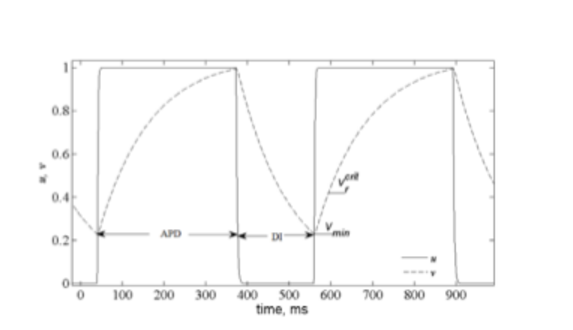
\includegraphics[width=.7\linewidth]{figure1.pdf} \\
            Source: Idris, et al (2012)
        \end{block}
      \end{column}
      \begin{column}{.48\linewidth}
        \begin{block}{CSC Model is Solvable}
            \begin{itemize}
                \item Chernyak-Starobin-Cohen (CSC) Model is exactly solvable, but tedious
                \item Instead we decouple the two variables by restricting \(u\) to the value of 0 or 1
                \item Approximate solution can now be found with a simple separation of variables of the total derivative
            \end{itemize}
        \end{block}

        \begin{block}{Separation of Variables}
            \centering
            \(\varepsilon \int dt = \int \frac{dv}{\zeta u + v_r -v}\)
        \end{block}

        \begin{block}{Sums Over QT and DI Intervals}
            \centering
            \(QT = \frac{1}{\varepsilon} ln[\frac{\zeta + v_r - v_{min}}{\zeta + v_r - 1}]\) \\[2ex]
            \(DI = \frac{1}{\varepsilon} ln[\frac{1-v_r}{v_{min}-v_r}]\)
        \end{block}
      \end{column}
    \end{columns}

    \begin{columns}
        \begin{column}{.98\linewidth}
            \begin{block}{Heart Intervals}
                \centering
                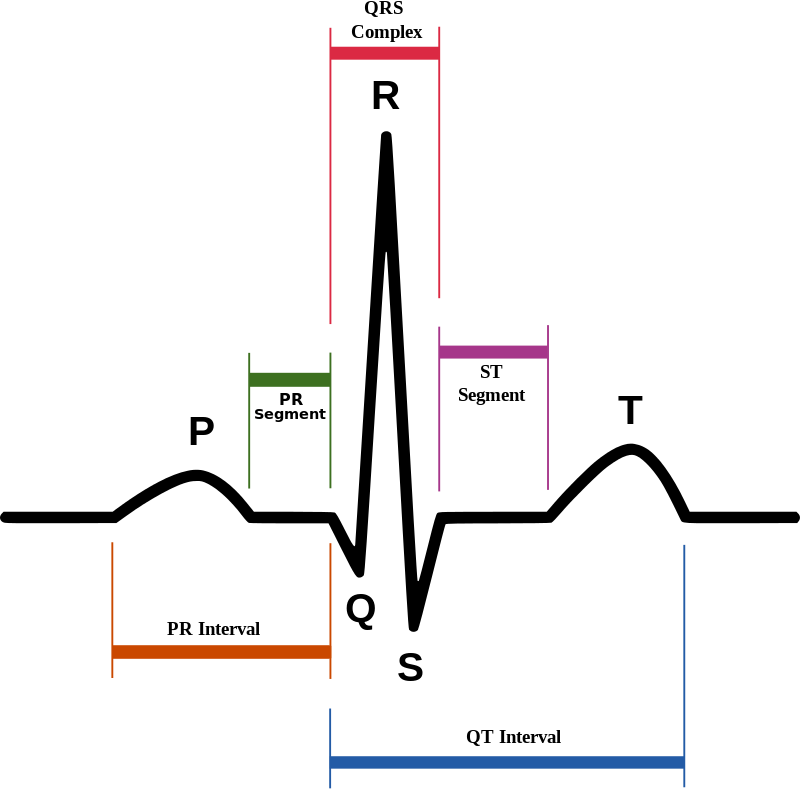
\includegraphics{qt.png} \\
                Source: Wikipedia User:Agateller
            \end{block}
        \end{column}
    \end{columns}

    \begin{columns}
        \begin{column}{.98\linewidth}
            \begin{block}{Application}
                \centering
                \begin{itemize}
                    \item There is a minimum membrane potential (\(v_{r}^{crit}\)) that \(v\) must drop below for another heart beat to start
                    \item Using an ECG measurement from a cardiac patient the ideal model can be fitted
                    \item Solving for the distance between \(v_r^{crit}\) and \(v_{min}\) predicts the chances of the membrane potential 
                        not reaching the minimum voltage for the next beat to start. This distance is called the Reserve 
                        of Refactoriness (RoR) \\[2ex]
                \end{itemize}
                \(RoR=\frac{v_r^{crit}-v_{min}}{v_r^{crit}}\)
            \end{block}
        \end{column}
    \end{columns}

    \begin{columns}
        \begin{column}{.98\linewidth}
            \begin{block}{Experimental Status}
                \centering
                \begin{itemize}
                    \item The paper \textit{Feasibility of Non-Invasive Determination of the Stability of Propagation Reserve in Patients} 
                        (2012) establishes the accuracy of the model compared to detailed heart measurements in healthy patients
                    \item Dr. Starobin's team is currently applying the model to analyze CNT toxicity in mice
                \end{itemize}
            \end{block}
        \end{column}
    \end{columns}
  \end{frame}
\end{document}


%%%%%%%%%%%%%%%%%%%%%%%%%%%%%%%%%%%%%%%%%%%%%%%%%%%%%%%%%%%%%%%%%%%%%%%%%%%%%%%%%%%%%%%%%%%%%%%%%%%%
%%% Local Variables: 
%%% mode: latex
%%% TeX-PDF-mode: t
%%% End:
